\documentclass[tikz,border=4pt]{standalone}
\usetikzlibrary{arrows.meta,positioning,calc,fit}
\begin{document}
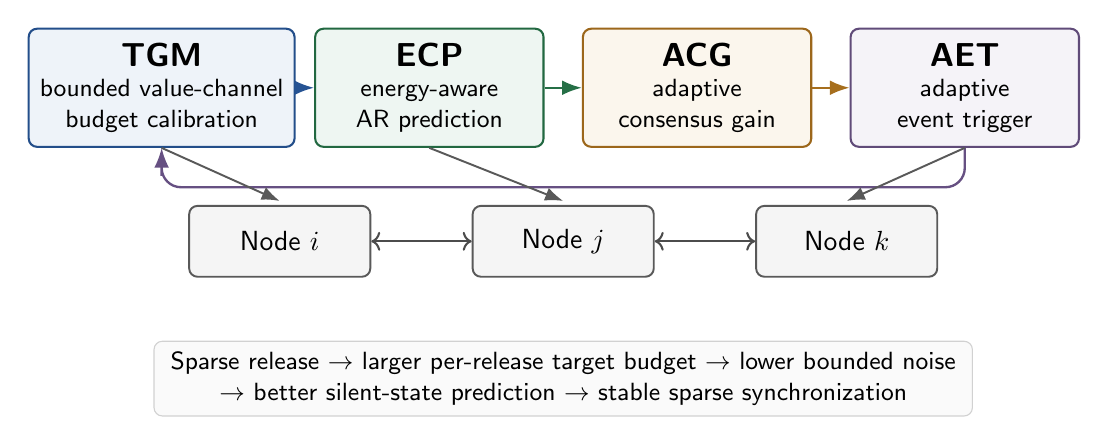
\begin{tikzpicture}[
  font=\sffamily,
  module/.style={draw=#1!75!black, fill=#1!8, rounded corners=3pt, line width=0.75pt,
    align=center, minimum width=29mm, minimum height=15mm, inner sep=4pt, font=\sffamily\small},
  nodebox/.style={draw=black!65, fill=black!4, rounded corners=3pt, line width=0.7pt,
    align=center, minimum width=23mm, minimum height=9mm, inner sep=3pt},
  arrow/.style={-{Latex[length=2.3mm]}, line width=0.7pt, draw=black!65},
  flow/.style={-{Latex[length=2.5mm]}, line width=0.85pt, draw=#1!80!black},
  label/.style={font=\sffamily\scriptsize, align=center, text=black!70}
]
\definecolor{EBlue}{HTML}{2F68B8}
\definecolor{EGreen}{HTML}{2E8B57}
\definecolor{EOrange}{HTML}{D08A24}
\definecolor{EPurple}{HTML}{8064A2}

\node[module=EBlue] (tgm) at (0,2.2) {\textbf{\large TGM}\\bounded value-channel\\budget calibration};
\node[module=EGreen] (ecp) at (3.4,2.2) {\textbf{\large ECP}\\energy-aware\\AR prediction};
\node[module=EOrange] (acg) at (6.8,2.2) {\textbf{\large ACG}\\adaptive\\consensus gain};
\node[module=EPurple] (aet) at (10.2,2.2) {\textbf{\large AET}\\adaptive\\event trigger};

\draw[flow=EBlue] (tgm) -- (ecp);
\draw[flow=EGreen] (ecp) -- (acg);
\draw[flow=EOrange] (acg) -- (aet);
\draw[flow=EPurple, rounded corners=7pt] (aet.south) |- ($(tgm.south)+(0,-0.50)$) -| (tgm.south);

\node[nodebox] (ni) at (1.5,0.25) {Node $i$};
\node[nodebox] (nj) at (5.1,0.25) {Node $j$};
\node[nodebox] (nk) at (8.7,0.25) {Node $k$};

\draw[arrow] (tgm.south) -- ($(ni.north)+(0,0.05)$);
\draw[arrow] (ecp.south) -- ($(nj.north)+(0,0.05)$);
\draw[arrow] (aet.south) -- ($(nk.north)+(0,0.05)$);
\draw[<->, line width=0.75pt, draw=black!70] (ni) -- (nj);
\draw[<->, line width=0.75pt, draw=black!70] (nj) -- (nk);

\node[draw=black!18, fill=black!2, rounded corners=3pt, inner xsep=6pt, inner ysep=4pt,
  font=\sffamily\small, align=center, below=8mm of nj] (loop)
  {Sparse release $\rightarrow$ larger per-release target budget $\rightarrow$ lower bounded noise\\
   $\rightarrow$ better silent-state prediction $\rightarrow$ stable sparse synchronization};
\end{tikzpicture}
\end{document}
